\experiment{Sparse Matrix}{04/10/2023}

\section{Aim}
To convert 2D matrix into sparse matrix, and perform addition operation and transpose operation
\section{Algorithm}
 {\fontfamily{lmtt}\selectfont
  \subsection{Convert to Sparse Matrix}
  Create a function \texttt{convert(m, n, matrix[m][n], terms[])}:
  \begin{enumerate}
    \item \textbf{Start}
    \item Initialize $k$, \texttt{row}, \texttt{column}, and \texttt{value}.
    \item Loop through matrix rows (\texttt{i}):
          \begin{enumerate}[label=2.\arabic*.]
            \item Loop through matrix columns (\texttt{j}):
                  \begin{enumerate}[label=2.1.\arabic*.]
                    \item If \texttt{matrix[i][j]} is non-zero:
                          Set \texttt{row}, \texttt{column}, and \texttt{value}.
                          Increment $k$.
                  \end{enumerate}
          \end{enumerate}
    \item Set \texttt{terms[0].row}, \texttt{terms[0].column}, and \texttt{terms[0].value}.
    \item \textbf{Stop}
  \end{enumerate}

  \subsection{Display Sparse Matrix}
  Create a function \texttt{display(terms[])}:
  \begin{enumerate}
    \item \textbf{Start}
    \item Print "Row\texttt{\textbackslash t}Column\texttt{\textbackslash t}Value".
    \item Loop through \texttt{terms} array (\texttt{i}):
          \begin{enumerate}[label=3.\arabic*.]
            \item Print \texttt{terms[i].row},\texttt{terms[i].column}, \texttt{terms[i].value}.
          \end{enumerate}
    \item \textbf{Stop}
  \end{enumerate}

  \subsection{Transpose Sparse Matrix}
  Create a function \texttt{transpose(terms[])}:
  \begin{enumerate}
    \item \textbf{Start}
    \item Initialize \texttt{transposed[terms[0].value]}.
    \item Loop through columns (\texttt{k}):
          \begin{enumerate}[label=2.\arabic*.]
            \item Loop through \texttt{terms} array (\texttt{i}):
                  \begin{enumerate}[label=2.1.\arabic*.]
                    \item If \texttt{terms[i].column} is equal to \texttt{k}:
                          Copy \texttt{terms[i]} to \texttt{transposed[i]}.
                  \end{enumerate}
          \end{enumerate}
    \item Call \texttt{display(transposed)}.
    \item \textbf{Stop}
  \end{enumerate}

  \subsection{Matrix Addition}
  Create a function \texttt{add(termsa[], termsb[])}:
  \begin{enumerate}[label=\arabic*.,left=0pt]
    \item \textbf{Start}
    \item Initialize \texttt{sum[MAX\_TERMS]}.
    \item Initialize \texttt{i}, \texttt{j}, and \texttt{k}.
    \item Loop while \texttt{i} $\leq$ \texttt{termsa[0].value}\ OR \texttt{j} $\leq$ \texttt{termsb[0].value}:
          \begin{enumerate}[label=4.\arabic*.]
            \item If \texttt{i} $\leq$ \texttt{termsa[0].value}\ AND \texttt{j} $\leq$ \texttt{termsb[0].value}:
                  \begin{enumerate}[label=4.1.\arabic*.]
                    \item If \texttt{termsa[i].row} $=$ \texttt{termsb[j].row}\ AND \texttt{termsa[i].column} $=$ \texttt{termsb[j].column}:
                          \begin{enumerate}[label=4.1.1.\arabic*.]
                            \item Set \texttt{sum[k].row}, \texttt{sum[k].column}, and \texttt{sum[k].value} as the sum of corresponding \newline values.
                            \item Increment \texttt{i} and \texttt{j}.
                          \end{enumerate}

                    \item Else if (\texttt{termsa[i].row} $<$ \texttt{termsb[j].row}) \newline
                          \hspace*{2em} OR (\texttt{termsa[i].row} $=$ \texttt{termsb[j].row} AND \texttt{termsa[i].column} $<$ \texttt{termsb[j].column}):
                          \begin{enumerate}[label=4.1.2.\arabic*.]
                            \item Set \texttt{sum[k]} as \texttt{termsa[i]}.
                            \item Increment \texttt{i}.
                          \end{enumerate}

                    \item Else:
                    \item Set \texttt{sum[k]} as \texttt{termsb[j]}.
                    \item Increment \texttt{j}.
                  \end{enumerate}
            \item Else if \texttt{i} $\leq$ \texttt{termsa[0].value}:
                  \begin{enumerate}[label=4.2.\arabic*.]
                    \item Set \texttt{sum[k]} as \texttt{termsa[i]}.
                    \item Increment \texttt{i}.
                  \end{enumerate}
            \item Else if \texttt{j} $\leq$ \texttt{termsb[0].value}:
                  \begin{enumerate}[label=4.3.\arabic*.]
                    \item Set \texttt{sum[k]} as \texttt{termsb[j]}.
                    \item Increment \texttt{j}.
                  \end{enumerate}
            \item Increment \texttt{k}.
          \end{enumerate}
    \item Loop end.
    \item Print "Sum:".
    \item Call \texttt{display(sum)}.
    \item \textbf{Stop}
  \end{enumerate}

  \subsection{Main}

  \begin{enumerate}[label=\arabic*.,left=0pt]
    \item \textbf{Start}
    \item Define a structure for a matrix term with row, column, and value fields.
    \item Define constant \texttt{MAX\_TERMS} as 101.\
    \item Define arrays \texttt{termsa[MAX\_TERMS]} and \texttt{termsb[MAX\_TERMS]} for sparse matrices.
    \item Initialize \texttt{ch} to 0.
    \item Print "Enter order of matrix a:".
    \item Read \texttt{m}, \texttt{n}.
    \item Initialize \texttt{int a[m][n]}.
    \item Print "Enter matrix a:".
    \item Read matrix \texttt{a}.
    \item Call \texttt{convert(m, n, a, termsa)}.
    \item Print "Enter order of matrix b:".
    \item Read \texttt{p}, \texttt{q}.
    \item Initialize \texttt{int b[p][q]}.
    \item Print "Enter matrix b:".
    \item Read matrix \texttt{b}.
    \item Call \texttt{convert(p, q, b, termsb)}.
    \item Print "Matrix A:".
    \item Call \texttt{display(termsa)}.
    \item Print "Matrix B:".
    \item Call \texttt{display(termsb)}.
    \item Call \texttt{add(termsa, termsb)}.
    \item Print "Transpose A:".
    \item Call \texttt{transpose(termsa)}.
    \item Print "Transpose B:".
    \item Call \texttt{transpose(termsb)}.
    \item \textbf{Stop}
  \end{enumerate}
 }

\section{C Program}

\begin{lstlisting}[label={list:c_program:sparse_matrix}]
#include <stdlib.h>
#include <stdio.h>

#define MAX_TERMS 101

typedef struct term
{
  int row, col, value;
} term;

term termsa[MAX_TERMS];
term termsb[MAX_TERMS];

void convert(int m, int n, int a[m][n], term terms[]);
void display(term terms[]);
void transpose(term terms[]);
void add(term termsa[], term termsb[]);

int main()
{
  int ch;
  printf("Enter order of matrix a: ");
  int m, n, p, q;
  scanf("%d %d", &m, &n);
  int a[m][n];
  printf("\nEnter matrix a:\n");
  for (int i = 0; i < m; i++)
  {
    printf("Enter row %d: ", i + 1);
    for (int j = 0; j < n; j++)
    {
      scanf("%d", &a[i][j]);
    }
  }
  printf("\nEnter order of matrix b: ");
  scanf("%d %d", &p, &q);
  int b[p][q];
  printf("\nEnter matrix b:\n");
  for (int i = 0; i < p; i++)
  {
    printf("Enter row %d: ", i + 1);
    for (int j = 0; j < q; j++)
    {
      scanf("%d", &b[i][j]);
    }
  }
  convert(m, n, a, termsa);
  convert(p, q, b, termsb);

  printf("\nMatrix A = \n");
  display(termsa);

  printf("\nMatrix B = \n");
  display(termsb);

  add(termsa, termsb);

  printf("\nTraspose A = :\n");
  transpose(termsa);
  printf("\nTraspose B = :\n");
  transpose(termsb);
}

void convert(int m, int n, int a[m][n], term terms[])
{
  int i, j, k = 1;
  terms[0].row = m;
  terms[0].col = n;
  terms[0].value = 0;
  for (i = 0; i < m; i++)
  {
    for (j = 0; j < n; j++)
    {
      if (a[i][j] != 0)
      {
        terms[k].row = i + 1;
        terms[k].col = j + 1;
        terms[k].value = a[i][j];
        k++;
      }
    }
  }
  terms[0].value = k - 1;
}

void display(term terms[])
{
  printf("\nRow\tColumn\tValue\n");
  for (int i = 0; i <= terms[0].value; i++)
  {
    printf("%d\t%d\t%d\n", terms[i].row, terms[i].col, terms[i].value);
  }
}

void transpose(term terms[])
{
  term transposed[terms[0].value];
  transposed[0].row = terms[0].col;
  transposed[0].col = terms[0].row;
  transposed[0].value = terms[0].value;
  for (int k = 1; k <= terms[0].col; k++)
  {
    for (int i = 1; i <= terms[0].value; i++)
    {
      if (terms[i].col == k)
      {
        transposed[i].col = terms[i].row;
        transposed[i].row = k;
        transposed[i].value = terms[i].value;
      }
    }
  }
  display(transposed);
}

void add(term termsa[], term termsb[])
{
  term sum[MAX_TERMS];
  sum[0].row = termsa[0].row;
  sum[0].col = termsa[0].col;
  sum[0].value = 0;
  int i = 1, j = 1, k = 1;
  while (i <= termsa[0].value || j <= termsb[0].value)
  {
    if (i <= termsa[0].value)
    {
      if (j <= termsb[0].value)
      {
        if (termsa[i].row == termsb[j].row)
        {
          if (termsa[i].col == termsb[j].col)
          {
            sum[k].row = termsa[i].row;
            sum[k].col = termsa[i].col;
            sum[k].value = termsa[i].value + termsb[j].value;
            i++;
            j++;
          }
          else if (termsa[i].col < termsb[j].col)
          {
            sum[k].row = termsa[i].row;
            sum[k].col = termsa[i].col;
            sum[k].value = termsa[i].value;
            i++;
          }
          else
          {
            sum[k].row = termsb[j].row;
            sum[k].col = termsb[j].col;
            sum[k].value = termsb[j].value;
            j++;
          }
        }
        else if (termsa[i].row < termsb[j].row)
        {
          sum[k].row = termsa[i].row;
          sum[k].col = termsa[i].col;
          sum[k].value = termsa[i].value;
          i++;
        }
        else
        {
          sum[k].row = termsb[j].row;
          sum[k].col = termsb[j].col;
          sum[k].value = termsb[j].value;
          j++;
        }
      }
    }
    else
    {
      sum[k].row = termsb[j].row;
      sum[k].col = termsb[j].col;
      sum[k].value = termsb[j].value;
      j++;
    }
    k++;
  }
  sum[0].value = k - 1;
  printf("\nSum:\n");
  display(sum);
}
\end{lstlisting}

\section{Output}

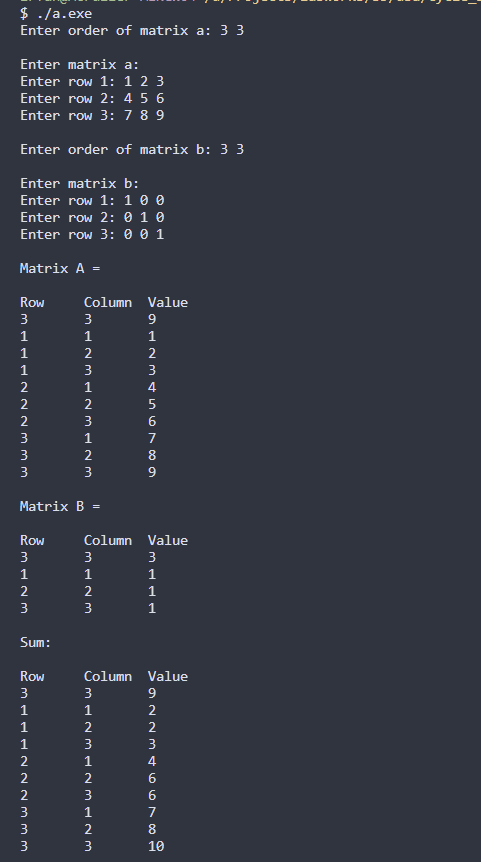
\includegraphics[]{Cycle_1/Outputs/SparseMatrix.png}
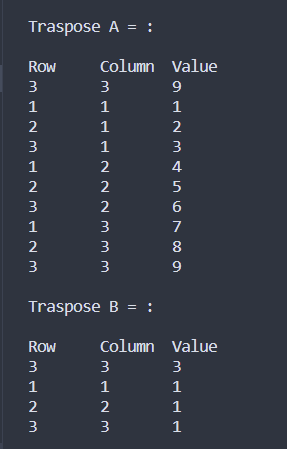
\includegraphics[]{Cycle_1/Outputs/SparseTranspose.png}

\section{Result}
Implemented sparse matrix conversion,addition and transpose.Program is executed successfully and output is verified.